\documentclass[12pt,letterpaper]{report}
\usepackage[utf8]{inputenc}
\usepackage[spanish]{babel}
\usepackage{amsmath}
\usepackage{amsfonts}
\usepackage{amssymb}
\usepackage{physics}
%\usepackage{cite}
\usepackage{graphicx}
\usepackage[table]{xcolor}
%\usepackage[usenames]{color}
\usepackage[draft,inline,nomargin]{fixme} \fxsetup{theme=color}
\FXRegisterAuthor{cc}{acc}{\color{green}CC}
\usepackage{wrapfig}
\usepackage{hyperref}
\usepackage{booktabs}
\usepackage[backend=bibtex,style=phys]{biblatex}
\bibliography{referencias}
\usepackage[left=2.5cm,right=2.5cm,top=2cm,bottom=2cm]{geometry}
\usepackage{setspace}

\begin{document}
\begin{titlepage}
	\begin{center}
	\LARGE
	Universidad de El Salvador \\ 
	Facultad de Ciencias Naturales y Matemática  \\
	Escuela de Física
	\end{center}
	
%	\vspace{0.5cm}

	\begin{figure}[h]
	\centering
	
\includegraphics[scale=0.08]{ues_logo.png}
	\end{figure}

%	\vspace{0.5cm}
	
	\begin{center}
	\Large
	Trabajo de Graduaci\'on	\\
	
%	\vspace{0.5cm}
	\LARGE
	\textit{\textbf{``Estudio de la componente mu\'onica en la distribuci\'on lateral de cascadas atmosf\'ericas"}}\\
	
	\vspace{2.0cm}
	\large
	Presentado por\\
	Cindy Mariella Castellón Salguero\\
	\vspace{0.8cm}
	\large
	Para optar al grado de\\
	Licenciada en F\'isica	
	
	\vspace{1.5cm}
	Asesores\\
	Ph. D. Hermes Le\'on Vargas\\
	M. Sc. Ra\'ul Antonio Henr\'iquez Ort\'iz\\
	
	\vspace{2.5cm}
	\textit{Ciudad Universitaria ``Dr. Fabio Castillo", mayo de 2022}
	\end{center}
\end{titlepage}
 
\tableofcontents
\listoffigures
\listoftables

\chapter*{Resumen}
\addcontentsline{toc}{chapter}{Resumen}
\spacing{1.5}


Uno de los principales problemas estudiados en la física de rayos cósmicos es el de la composición primaria de los rayos cósmicos que entran a la atmósfera terrestre con ultraaltas energías ($>10^{17}$ eV). La colaboración Pierre Auger propone una composición mixta que contiene fracciones de elementos con masas que se encuentran entre la del hidrógeno y la del hierro. Se ha verificado el impacto de la composición mixta propuesta sobre observables de los chubascos atmosféricos, como la profundidad del máximo. También se ha estudiado el efecto de la composición primaria en las distribuciones laterales de electrones y muones, así como en su densidad a cierta distancia. Lo anterior se ha hecho realizando simulaciones de dichos eventos con el programa AIRES utilizando tres modelos distintos de interacciones hadrónicas de altas energías. Se han comparado los resultados de profundidad del máximo con datos del Observatorio Pierre Auger, apoyando la hipótesis de una composición mixta. Se observó en la mayoría de casos que el efecto de la masa de la partícula primaria en las distribuciones laterales es evidente a cortas distancias del eje del chubasco pero las diferencias disminuyen a medida la distancia crece. Similarmente se aprecia que al aumentar la energía primaria, las distribuciones laterales de muones se vuelven indistinguibles; ajustes a una función de tipo NKG ilustran estas dependencias así como las diferencias entre los modelos, de los cuales QGSJETII-04 es el que más discrepa de los otros. Por otro lado, los resultados de densidad de electrones a $r_{opt}$ muestran ser independientes de la composición primaria, mientras que la de muones sí muestra una pequeña dependencia; ambas siendo independientes del modelo hadrónico. 

 
\singlespacing

\chapter*{Introducción}
\addcontentsline{toc}{chapter}{Introducción}
%%%%%Historia/definiciones
\spacing{1.25}
Los rayos cósmicos -descubiertos por el austríaco Victor Hess en 1914- son partículas cargadas provenientes del exterior de la Tierra que llegan a la misma con energías de hasta $10^{20}$ eV. Éstos son en su mayoría protones (90\%) y núcleos de helio (9\%), el resto son electrones, positrones y núcleos más pesados. Cuando los rayos cósmicos entran a la atmósfera terrestre interactúan con los átomos y moléculas de la misma, generando cascadas de partículas secundarias que se conocen como chubascos atmosféricos, éstos son producto de interacciones electromagnéticas y hadrónicas. \\

Desde el descubrimiento de los rayos cósmicos, se han estudiado ampliamente aspectos como su espectro, su composición, su propagación y su origen. Se conoce que el espectro de rayos cósmicos se extiende desde $10^9$ hasta $10^{20}$ siguiendo una ley de potencias, y que a estas ultraaltas energías se observa una supresión del mismo. También se ha concluido que los rayos cósmicos están compuestos mayormente por protones, y que sus fuentes son principalmente de origen galáctico. Sin embargo las interrogantes fundamentales de la física de rayos cósmicos, relacionadas con su origen y el mecanismo de aceleración con el que alcanzan las energías observadas, siguen vigentes. \\

%%%%%Problema (sim vs obs) (composition problem)
En particular el rango de las ultraaltas energías presenta grandes desafíos para la investigación en esta área. Esto debido principalmente a limitaciones experimentales relacionadas con el bajo flujo de partículas a estas energías, así como limitaciones teóricas en la descripción de las interacciones hadrónicas, ya que los modelos utilizados son fenomenológicos y dependen de los avances en aceleradores de partículas. Actualmente uno de los problemas esenciales es la determinación de la composición de los rayos cósmicos de ultraaltas energías. El problema de la composición consiste en dar una correcta interpretación a los datos observacionales basada en simulaciones de chubascos. \\

Se han medido con bastante precisión diversas propiedades de los chubascos producidos por rayos cósmicos de ultraalta energía que son especialmente sensibles a la composición primaria, no obstante no se ha logrado una interpretación coherente de dichas mediciones en términos de una única composición. Existen importantes discrepancias entre las simulaciones con distintos modelos de interacción hadrónica, de manera que dirigen a conclusiones no compatibles entre sí, y además no compatibles con las observaciones realizadas de las magnitudes dependientes de la composición.\\

%%%%%Objetivo del trabajo  
El objetivo de este trabajo de investigación es verificar el efecto de una composición mixta de los rayos cósmicos de ultraalta energía en las observables $X_{max}$ y $\sigma X_{max}$ -que son sensibles a la masa de la partícula inicial-, así como estudiar su efecto en la distribución lateral de electrones y muones. Esto pretende lograrse realizando simulaciones de chubascos atmosféricos tomando en cuenta una composición que no sea completamente ligera ni únicamente pesada y comparando los resultados con datos medidos y publicados por la colaboración Pierre Auger. Además se pretende comparar los resultados obtenidos de simulaciones realizadas con diferentes modelos de interacciones hadrónicas, en este caso: Sibyll 2.3c, EPOS-LHC y QGSJETII-04. \\

%%%%%¿Cómo se hizo? 
Se realizaron simulaciones de 2400 eventos de chubascos atmosféricos iniciados por protones, núcleos de helio, núcleos de nitrógeno y núcleos de hierro con energías iniciales entre $180.30$ PeV a $42.267$ EeV. El \textit{software} utilizado para simular los chubascos fue AIRES, que cuenta con los modelos hadrónicos como paquetes externos, además de una librería de módulos escritos en Fortran y C++ para realizar los cálculos de las características de los eventos simulados. Adicionalmente, los datos observacionales fueron tomados del repositorio que se encuentra en sitio web del Observatorio Pierre Auger. \\

%%%%%Capítulos
En el capítulo 1 se resume el fundamento teórico necesario para la comprensión física de los chubascos atmosféricos producidos por rayos cósmicos y sus propiedades principales, así como el estado del conocimiento del tema. El capítulo 2 describe el programa AIRES utilizado para las simulaciones, así como las condiciones que se asumen para las mismas. En el capítulo 3 se presentan los resultados obtenidos de las simulaciones y se realiza una comparación entre los modelos hadrónicos, así como con los datos experimentales correspondientes.




\singlespace

\chapter{Marco teórico}
\spacing{1.25}
%\vspace{-5mm}
\section{Rayos Cósmicos}
Los rayos cósmicos (RC) son partículas cargadas aceleradas a altas energías que se propagan por el espacio y llegan a la atmósfera terrestre. En una primera aproximaci\'on de todo el espectro de RC un $90\%$ de estas partículas son protones, un $9\%$ núcleos de helio y el resto son electrones, núcleos más pesados y antipartículas. La mayoría de RC son relativistas; su espectro de energías está entre $\sim 10^9$ y $\sim 10^{20}$ eV, y sigue una ley de potencias. Actualmente se tiene conocimiento de fuentes de RC de origen galáctico y extragaláctico \cite{Gaisser1990}. A continuación se describen algunos aspectos del desarrollo histórico de la investigación sobre los RC.
	
	\subsection{Descubrimiento y naturaleza de los RC}
	En el año 1900 se realizaban experimentos para estudiar la ionización causada por elementos radiactivos, en estos se observó que el aire contenía algún tipo de radiación que también era capaz de ionizar. A partir de esto se inició la búsqueda del origen de dicha radiación. Se repitieron los experimentos a alturas de $300$ a $1300$ m, esperando que si la fuente de la radiación fuese la corteza terrestre, ésta disminuiría con la altura. En 1911-1912, el austriaco Victor Hess realizó experimentos en globo a alturas de hasta $5200$ m, con los que concluyó que la radiación debía originarse fuera de la Tierra y que, comparando mediciones de día y de noche, no provenía del sol. Victor Hess es considerado el descubridor de los rayos cósmicos \cite{Extremas}.\\
	
	Posteriormente se inició la búsqueda de la naturaleza de estas partículas, siendo el candidato más popular los rayos gamma. En 1927 Jacob Clay observó una disminución de la radiación en bajas latitudes. Esto fue explicado en 1932 por Arthur Compton como la acción del campo magnético de la Tierra sobre los RC, llevando a la conclusión de que la mayor parte de las partículas en cuestión debían tener carga eléctrica, y estudiando los efectos geomagnéticos este-oeste se dedujo que casi todas las cargas eran positivas. Finalizando la década de 1940, experimentos de detección directa realizados por Schein establecieron que aproximadamente el $99\%$ de los RC son protones, núcleos de Helio y núcleos más pesados y que sólo el $1\%$ son electrones, positrones y rayos gamma \cite{Dorman2004}.

	\subsection{Producción de RC}		
	En la figura \ref{fig:espectro} se muestra el espectro observado de RC, el cual está bien representado por una ley de potencias:
	\begin{align}
	\dv{N}{E}=E^{-(\gamma+1)}.
	\end{align}	
	El índice $\gamma$ tiene un valor aproximadamente constante de $2.7$ con dos ligeros cambios: uno a $\sim 10^{16}$ eV, conocido como la \textit{rodilla}, y el otro a $\sim 10^{19}$ eV conocido como el \textit{tobillo} \cite{Extremas}. El espectro se extiende desde  $\sim 10^9$ hasta $\sim 10^{20}$ eV.
	
	\begin{figure}[h]
	\centering	
	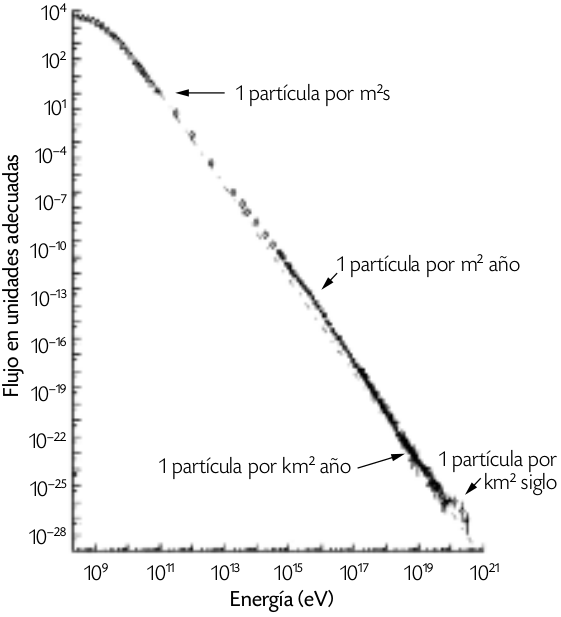
\includegraphics[width=0.5\textwidth]{Figuras/espectro_RC} 
	\caption{Intensidad del flujo de rayos cósmicos en función de su energía. Éste está bien representado por una ley de potencias $E^{-2.7}$. (Tomada de \cite{Poderosas}).}
	\label{fig:espectro}
	\end{figure}	

	Por tanto, debe haber un mecanismo capaz de acelerar partículas a tales energías y que reproduzca la forma del espectro observado. En 1949, Fermi propuso un mecanismo en el que las partículas podían ganar energía en colisiones estocásticas en regiones del espacio donde existiesen campos magnéticos turbulentos, como las ondas de choque resultado de un colapso gravitacional, por ejemplo. Se considera que una partícula de prueba tiene un incremento de energía proporcional a la misma $\Delta E = \xi E$ en cada colisión, luego de $n$ colisiones la energía de la partícula será \cite{Gaisser1990}
	\begin{align}
	E_n = E_0 \qty(1+\xi)^n,
	\end{align}
donde $E_0$ es la energía con la que entra al proceso de aceleración. Tomando en cuenta la probabilidad $P_{esc}$ de que la partícula escape de la región de aceleracón, la proporción de partículas que se aceleran a energías mayores a un valor $E$ es
	\begin{align}
	N(\geq E) \propto \frac{1}{P_{esc}}\qty(\frac{E}{E_0})^{-\gamma},
	\end{align}
	con $\gamma = -\ln(1-P_{esc})/\ln(1+\xi) \approx P_{esc}/\xi$, de manera que este mecanismo efectivamente reproduce la ley de potencias que caracteriza al espectro de RC. \\
	
	El mecanismo de Fermi se describe en dos situaciones físicas: nubes de plasma magnetizadas (aceleración de Fermi de segundo orden) y frentes de onda de choque (aceleración de Fermi de primer orden). En la aceleración de segundo orden se considera una partícula que entra a la nube con cierta velocidad, donde cambia su dirección de modo aleatorio por interacciones con el campo magnético turbulento en el interior, mediante este proceso se tiene $\xi=(4/3) \beta^2$, donde $\beta= V/c$ es la velocidad de la nube; en la aceleración de primer orden se considera que la partícula atraviesa la onda de choque e interactúa con el campo magnético del gas que éste va dejando detrás (\textit{downstream}), en este caso $\xi=(4/3) \beta$, donde $\beta= V/c$ se refiere la velocidad del gas detrás del choque respecto al gas delante del choque (\textit{upstream}).
	
	\subsection{Fuentes de RC}
	Luego de establecer cómo pueden acelerarse las partículas, se buscaron objetos astronómicos que cumplan las condiciones necesarias para que el proceso se lleve a cabo. Para que el proceso sea eficaz, la partícula debe estar contenida en una región de radio $R$, tal que se cumpla la siguiente relación \cite{DeAngelis2015}:	
	\begin{align}
	E[\text{PeV}] \simeq B[\mu\text{G}]\times R[\text{pc}].
	\end{align}
	Ésta es llamada relación de Hillas, ilustrada en la figura \ref{fig:Hillas}, en la que también pueden observarse los potenciales aceleradores. Como fuentes de RC de origen galáctico pueden mencionarse las estrellas de neutrones de rápida rotación (púlsares) y los remanentes de supernova, mientras que en el caso extragaláctico se consideran los núcleos galácticos activos y los destellos de rayos gamma.
	
	\begin{figure}[h]
	\centering	
	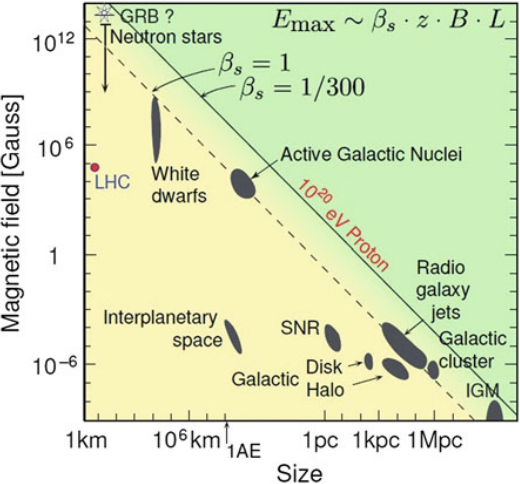
\includegraphics[width=0.5\textwidth]{Figuras/Hillas_Relation} 
	\caption{La gráfica de Hillas representa las potenciales fuentes de rayos cósmicos según la intensidad de su campo magnético y su tamaño. (Tomada de \cite{DeAngelis2015}).}
	\label{fig:Hillas}
	\end{figure}	

	\subsection{Propagación de RC}
	La presencia de campos magnéticos en el espacio limita la posibilidad de estudiar las fuentes de RC a través de ellos. Los RC llegan a la Tierra isotrópicamente; llegan de todas direcciones con la misma frecuencia, lo que sugiere una trayectoria casi aleatoria desde la fuente hacia la Tierra. Dentro de la galaxia las partículas pueden sufrir varios procesos: difusión en campos magnéticos, convección por vientos galácticos, pérdidas o ganancias de energía, colisiones nucleares con gas interestelar y decaimientos. Para describir la propagación de RC debe resolverse la ecuación de transporte \cite{Gaisser1990}:
	\begin{align}
	\pdv{\mathcal{N}}{t} &= \nabla \cdot \qty(D_i \nabla \mathcal{N}_i)-\pdv{E} \qty[b_i(E)\mathcal{N}_i(E)]-\nabla \cdot u \mathcal{N}_i(E) \nonumber \\
	&+ Q_i(E,t) - p_i \mathcal{N}_i + \frac{v \rho}{m} \sum_{k \geq i}\int \frac{\dd \sigma_{i,k}\qty(E,E')}{\dd E}\mathcal{N}_k(E')\dd E',
	\end{align}
	que contempla los procesos mencionados para calcular la densidad de partículas con energías entre $E$ y $E+\dd E$. Los seis términos de la ecuación representan, respectivamente: la difusión, ganancias de energía, convección, la inyección de partículas, pérdida de partículas por colisiones o decaimientos, cascadas de decaimientos o fragmentación nuclear. 

\section{Interacciones de los RC}
	\subsection{Interacciones electromagnéticas}
	Las partículas cargadas en general interactúan con átomos; estas pueden ionizarlos, excitarlos o producir fotones. Para electrones y positrones a altas energías es relevante la radiación de frenado o \textit{bremsstrahlung}, en la cual partículas cargadas emiten radiación al ser deflectadas por el campo eléctrico de los átomos en un medio. En este proceso, la fracción de energía que la partícula pierde puede describirse por \cite{DeAngelis2015}:
	\begin{align}
	\frac{1}{E} \dv{E}{x} \simeq -\frac{1}{X_0},
	\end{align}
	donde $X_0$ es la longitud de radiación que es dependiente del medio.\\
	
	Por otro lado, los fotones interactúan con un medio principalmente mediante efecto fotoeléctrico (emisión de un electrón de un material que ha absorbido un fotón), dispersión de Compton (transferencia de energía de un fotón hacia un electrón mediante una colisión) y producción de pares electrón-positrón. Este último proceso siendo el más relevante a altas energías; al interactuar con el campo eléctrico de un núcleo, el fotón tiene cierta probabilidad de formar un par $e^{-}-e^{+}$, con una longitud de interacción:
	\begin{align}
	\lambda \simeq \frac{9}{7} X_0.
	\end{align}	
	Los fotones también puede sufrir otros procesos como dispersión de Rayleigh, que puede tener importancia para el transporte de la luz a través de la atmósfera, o interacciones fotonucleares (excitación de núcleos) que se dan a energías alrededor de $10$ MeV.
	
	\subsection{Interacciones hadrónicas}
	Los RC primarios están mayoritariamente conformados por hadrones, como lo son los protones y núcleos. Los hadrones se describen mediante el modelo de quarks \cite{DeAngelis2015}, partículas que interactúan mediante la interacción nuclear fuerte y que, según observaciones, no existen de manera aislada sino en estados ligados de dos o tres quarks. Este tipo de modelos se estudian desde la \textit{cromodinámica cuántica} (QCD por sus siglas en inglés), donde se propone el concepto de \textit{color} como la carga que origina las interacciones fuertes, y el de \textit{gluón} como la partículas mediadora. \\
		
	\begin{wrapfigure}{r}{0.3\textwidth}
	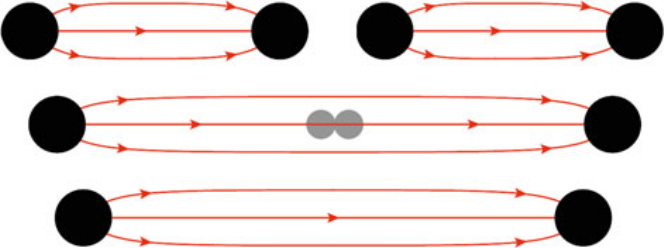
\includegraphics[width=0.3\textwidth]{Figuras/string_frag} 
	\caption{De abajo hacia arriba; fragmentación de una cuerda creando un nuevo par de quarks en el campo de color. (Tomada de \cite{DeAngelis2015}).}
	\label{fig:string}
	\end{wrapfigure}		
	
	Para describir las interacciones hadrónicas se necesitan modelos fenomenológicos apoyados en QCD. Un modelo usado comúnmente es el modelo de cuerdas de Lund (o \textit{string model}) \cite{FragModels}; cuando los hadrones interactúan se forma un campo de color (cuerda) entre pares quark-antiquark, la energía potencial en dicha cuerda aumenta hasta fragmentarse y formar otros quarks que a su vez pueden formar hadrones, como se ilustra en la figura \ref{fig:string}. También suele utilizarse el modelo de \textit{minijet}, para tomar en cuenta la multiplicidad de partículas producidas. \\

	Actualmente existen varios generadores Monte Carlo de eventos hadrónicos; describen este tipo de interacciones basándose en diferentes modelos para ciertos aspectos de la interacción y en datos de colisionadores de partículas. Ejemplos de estos son SIBYLL \cite{Riehn2020}, QGSJET \cite{Ostapchenko2011} y EPOS \cite{Pierog2015}, que están especializados en interacciones de altas energías. 
	

\section{Cascadas atmosf\'ericas}
	Una cascada (tambi\'en llamada chubasco) atmosf\'erica (español para \textit{Air Shower}) es una cascada de partículas generada por la interacción de un rayo cósmico en la alta atmósfera. Antes de profundizar en cómo se desarrollan estas cascadas, conviene describir brevemente las principales características de la atmósfera.
	
	\subsection{Atmósfera terrestre}
	La capa de aire que rodea la Tierra se extiende hasta una altura  mayor a $100$ km. Según el modelo \textit{US Standard Atmosphere}, la atmósfera está compuesta principalmente por N$_2$ ($78$ \%), O$_2$ ($21$ \%) y Ar ($0.9$ \%). Acorde al mismo modelo, la densidad del aire es función de la altura:
	\begin{align}
	\rho(h)=\rho_0 e^{-\frac{h}{h_a}},
	\end{align}
	donde $\rho_0 = 1.22\times 10^{-3}$ g/cm$^3$ y $h_a = 8.2$ km. Sin embargo, en el estudio de los chubascos atmosféricos es más frecuente utilizar el concepto de \textit{profundidad} en lugar de la altura. La profundidad $X$ indica la cantidad de materia que atraviesa una partícula al moverse de un punto a otro. Esta se relaciona con la densidad mediante:
	\begin{align}
	X = \int_h^{\infty} \rho (h) \dd h.
	\end{align}

	\subsection{Desarrollo de una cascada atmosférica}	
	Las cascadas atmosf\'ericas se desarrollan de forma compleja como una combinación de cascadas electromagnéticas y producción de partículas por interacciones hadrónicas \cite{Matthews2005}. A grandes rasgos, una interacción hadrónica entre el rayo cósmico primario y un núcleo de la atmósfera produce múltiples partículas secundarias: una partícula principal (con la mayor parte de la energía inicial) que puede iniciar otro chubasco, y un gran número de mesones, principalmente piones cargados ($\pi^{\pm}$) y neutros ($\pi^0$).\\

	La componente electromagnética de la cascada es generada por los piones neutros al decaer en fotones ($\pi^0 \rightarrow \gamma \gamma$), esta cascada consiste en producción de pares ($\gamma\rightarrow e^+ e^-$) y bremsstrahlung ($e^{\pm} \rightarrow e^{\pm}\gamma$). Por su parte, los piones cargados pueden volver a interactuar hadrónicamente mientras tengan suficiente energía, luego de eso decaerán en neutrinos y muones ($\pi^{-} \rightarrow \mu^- \bar{\nu}_{\mu}$, $\pi^{+} \rightarrow \mu^+ \nu_{\mu} $). El desarrollo de un chubasco se ilustra en la figura \ref{fig:airshower}.\\
				
	\begin{figure}[h]
	\centering
	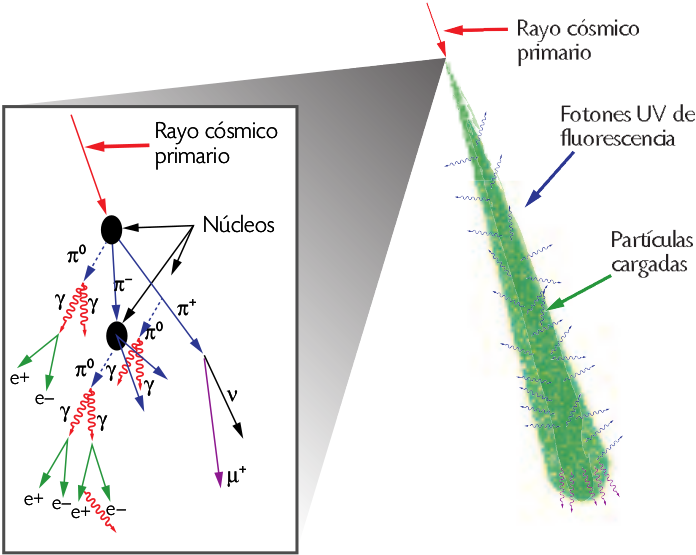
\includegraphics[width=0.6\textwidth]{Figuras/air_shower} 
	\caption{Esquema de la formación y desarrollo de un chubasco atmosférico. Se observa la componente hadrónica y la electromagnética. (Tomada de \cite{Poderosas}).}
	\label{fig:airshower}
	\end{figure}	
	
	La propagación de partículas (nucleones en particular) a través de la atmósfera, puede describirse con la ecuación de cascada:
	\begin{align}
	\dv{N(E,X)}{X} = -\frac{N(E,X)}{\lambda_N(E)} + \int_E^{\infty}\frac{N(E',X)}{\lambda_N(E)} F_{NN}(E,E') \frac{\dd E'}{E},
	\end{align}
	donde $N(E,X) \dd E$ es el flujo de nucleones a una profundidad $X$ en la atmósfera con energías entre $E$ y $E+\dd E$, $\lambda_N$ es la longitud de interacción del nucleón en el aire y $F_{NN}$ es la sección eficaz para la colisión de un nucleón incidente de energía $E'$ con un núcleo del aire, produciendo otro nucleón con energía $E$. Para generalizar al caso de la propagación de los múltiples hadrones producidos, se considera un grupo de ecuaciones acopladas \cite{Gaisser1990}:
	\begin{align}
	\dv{N_i(E,X)}{X} = -\qty(\frac{1}{\lambda_i}+\frac{1}{d_i}) N_i(E,X) + \sum_i \int \frac{F_{ij}(E_i,E_j)}{E_i} \frac{N_j(E_j)}{\lambda_j} \dd{E_j}.
	\end{align}

		\subsubsection*{Modelo Heitler-Matthews}
		En 1954, W. Heitler presentó un modelo simplificado del desarrollo de la componente electromagnética, posteriormente modificado por J. Matthews. Aunque no reemplaza simulaciones detalladas de cascadas, el modelo Heitler-Matthews permite describir correctamente características importantes de las mismas. En el modelo de Heitler se describe la componente electromagnética como ilustra la figura \ref{fig:heitler_em}; 
		\begin{wrapfigure}{l}{0.3\textwidth}
		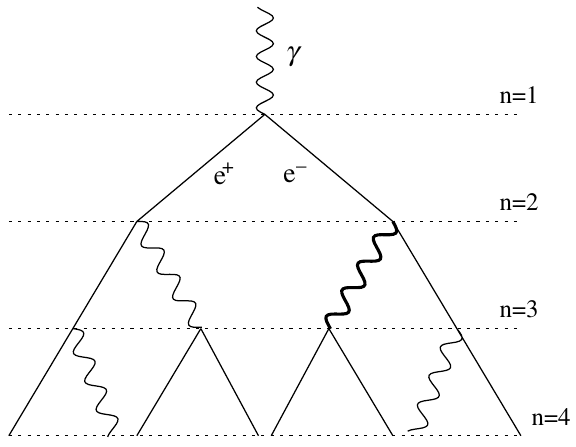
\includegraphics[width=0.3\textwidth]{Figuras/heitler_em.png} 
		\caption{Esquema de un chubasco puramente electromagnético; las líneas rectas representan electrones y las curvas representan fotones.}
		\label{fig:heitler_em}
		\end{wrapfigure}		
		luego de viajar una distancia $d=\lambda_r \ln 2$ (donde $\lambda_r$ es la longitud de radiación en el aire) un electrón produce un fotón que al viajar la misma distancia produce un par $e^- e^+$. Luego de $n$ divisiones, en la cascada hay un total de $N=2^n$ partículas; la división se detiene cuando las partículas alcanzan una energía crítica $\xi^e_c$. \\
		
		A partir de lo anterior pueden deducirse características de una cascada iniciada por un fotón:
		\begin{align}
		E_0 &= \xi ^e_c N_{\text{max}} \label{e0_em}, \\
		X^{\gamma}_{\text{max}} &= n_c \lambda \ln 2 = \lambda \ln[E_0/\xi ^e_c] \label{xmax_em},
		\end{align}
		donde $n_c$ es el número de longitudes $d$ necesarias para que la energía por partícula se reduzca a $\xi_c^e$, donde $N = N_{\text{max}}= 2^{n_c}$. Se observa que el número de partículas en el máximo aumenta linealmente con la energía inicial y que la profundidad aumenta con la energía de manera logarítmica.
		\begin{wrapfigure}{r}{0.3\textwidth}
		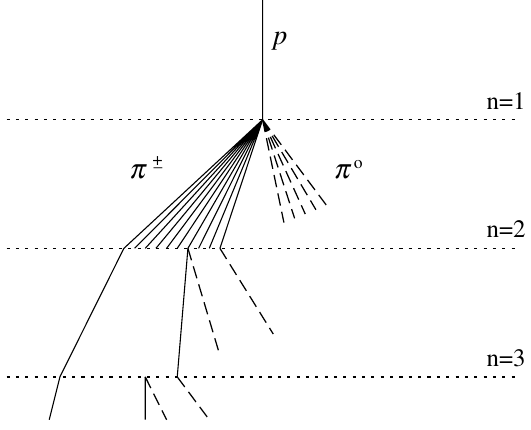
\includegraphics[width=0.3\textwidth]{Figuras/heitler_h.png} 
		\caption{Esquema de un chubasco producido por un protón; las líneas sólidas representan piones cargados mientras las líneas cortadas representan piones neutros.}
		\label{fig:heitler_h}
		\end{wrapfigure}	 
		Los chubascos iniciados por hadrones se describen similarmente, como se ilustra en la figura \ref{fig:heitler_h}. Se consideran capas de atmósfera de altura $\lambda_I \ln 2$ donde $\lambda_I$ es la longitud de interacción. Luego de atravesar una capa, un hadrón interactúa produciendo partes iguales de piones cargados y neutros; $N_{\pi^{\pm}}$ cargados y $N_{\pi^{0}}=\frac{1}{2}N_{\pi^{\pm}}$ neutros. Los piones cargados pueden repetir el proceso hasta alcanzar una energía crítica $\xi_c^{\pi}$, entonces se asume su decaimiento. \\
		
		Luego de $n$ capas, la energía por pion cargado es
		\begin{align}
		E_{\pi} = \frac{E_0}{\qty(\frac{3}{2}N_{\pi^{\pm}})^n},
		\end{align}
		de manera que el número de interacciones $n_c$ necesarias para que la energía por pion alcance el valor crítico es
		\begin{align}
		n_c = \frac{\ln \qty[E_0 / \xi_c^{\pi}]}{\ln \qty[\frac{3}{2}N_{\pi^{\pm}}]}.
		\end{align}
		Considerando una cascada iniciada por un protón, con componentes electromagnética y hadrónica, y tomando en cuenta el decaimiento de todos los piones en muones ($(N_{\pi^{\pm}}^{n_c} = N_{\mu}$) la energía total es
		\begin{align} \label{totalEnergy}
		E_0 = \xi_c^e N_{\text{max}}+\xi_c^{\pi} N_{\mu}.
		\end{align}
		El modelo de Heitler sobreestima la razón de electrones a fotones, de manera que se introduce un factor de corrección $g=10$ tal que $N_e = N/g$. Con esta corrección la ecuación (\ref{totalEnergy}) se reescribe como
		\begin{align} \label{e0_h}
		E_0 = g \xi_{c}^{e} \qty(N_e + \frac{\xi_c^{\pi}}{g \xi_c^{e}} N_{\mu}),
		\end{align}
		lo que indica que la energía inicial puede calcularse si se miden el número de electrones y de muones. Cabe mencionar que esta expresión es independiente del tipo de partícula primaria. Asimismo se puede estimar la profundidad del máximo $X_{\text{max}}^{p}$ tomando en cuenta que el protón primario interactúa a una profundidad $X_0=\lambda_I \ln 2$ como
		\begin{align} \label{xmax_h}
		X_{\text{max}}^{p} &= X_0 + \lambda_r \ln \qty[\frac{E_0}{3 N_{\pi^{\pm}}\xi_c^e}].
		\end{align}
		El segundo término corresponde a la profundidad del máximo de la componente electromagnética de la ecuación (\ref{xmax_em}), cuya energía inicial es $E_0/3N_{\pi^{\pm}}$. En las ecuaciones (\ref{e0_h}) y (\ref{xmax_h}) se observa que la dependencia del número de partículas y la profundidad del máximo con la energía inicial es líneal y logarítmica, respectivamente, tal como en (\ref{e0_em}) y (\ref{xmax_em}). En general los valores calculados con la ecuación (\ref{xmax_h}) son bastante bajos comparados con resultados de simulaciones; esto debido a que sólo se toma en cuenta la primera generación de partículas de la componente electromagnética. Por otro lado, el número de muones en la cascada puede expresarse en función de la energía como
		\begin{align}
		N_{\mu} &= \qty(\frac{E_0}{\xi_c^{\pi}})^{\beta}, \text{ donde } \beta = \frac{\ln[N_{\pi^{\pm}}]}{\ln[\frac{3}{2}N_{\pi^{\pm}}]}.
		\end{align}

	Para describir chubascos producidos por un núcleo $A$, en el modelo Heitler-Matthews se utiliza el modelo de superposición; se trata el núcleo como $A$ protones iniciando cascadas individualmente, cada uno con una porción igual de la energía inicial del núcleo $E_0$, es decir $E_0/A$. Las características de estas cascadas pueden obtenerse sustituyendo la energía inicial en las ecuaciones para protones, a la vez que se expresan en términos de las cantidades correspondientes a un chubasco producido por un protón de energía $E_0$, por ejemplo el número de muones y la profundidad del máximo puede expresarse como
	\begin{align}
	N_{\mu}^{A}		  	&= N_{\mu}^{p} A^{\beta -1}, \label{eq:NmuA} \\ 
	X_{\text{max}}^{A} 	&= X_{\text{max}}^{p} - \lambda_r \ln A. \label{eq:XmaxA}
	\end{align}

	Adicionalmente, Matthews presenta el modelo tomando en cuenta la inelasticidad de las interacciones; como resultado de una interacción se produce una partícula principal que se lleva la mayor parte de la energía, de manera que hay menos energía disponible para la producción de las múltiples partículas restantes. La inelasticidad se introduce con un parámetro $\kappa$ representando la porción de la energía inicial que se invierte en la producción de piones. Todas las expresiones anteriores corresponden a un valor $\kappa = 1$.

	
	\subsection{Métodos de observación}
	Se han diseñado experimentos con distintos principios para la observaci\'on de cascadas; \'estos pueden ser de \textit{radiación de Cherenkov}, como el \textit{High-Altitude Water Cherenkov Gamma-Ray Observatory} (HAWC) que detectan radiación producida por una partícula cargada que se mueve a través de un medio más rápido que la velocidad de la luz en ese medio; y de \textit{fluorescencia}, que colectan la luz emitida por las moléculas de nitrógeno excitadas en el chubasco, este método permite reconstruir el desarrollo longitudinal del mismo. Existen también observatorios híbridos, como el \textit{Telescope Array} (TA) y el \textit{Pierre Auger Observatory} (PAO); estos utilizan la técnica de fluorescencia para observar el desarrollo de la cascada y además detectan partículas de alta energía que alcanzan el nivel del suelo.
	
\section{Estado del conocimiento}
%Outline:
%- Preguntas abiertas en la fisica de rayos cosmicos

En la f\'isica de rayos c\'osmicos las preguntas fundamentales est\'an relacionadas con su origen y el mecanismo por el cu\'al adquieren su energ\'ia. Para energ\'ias cercanas a los TeV, los rayos c\'osmicos pueden detectarse directamente desde observatorios espaciales, sin embargo a medida que la energ\'ia aumenta y su flujo disminuye es necesaria la detecci\'on indirecta por medio de la observaci\'on de cascadas atmosf\'ericas desde el suelo. A partir de estas observaciones se recopilan las caracter\'isticas de los rayos c\'osmicos que pueden luego confrontarse con modelos te\'oricos para inferir informaci\'on sobre su origen. \\

%- Rayos cosmicos en el rango de los TeV
En la actualidad, los RC de ultraalta energía (UHECR, $E > 10^{18}$ eV) siguen considerándose un enigma en términos de su composición y origen. Experimentos como TA y PAO miden observables de las cascadas, entre ellas $X_{max}$, $X_{max}^{\mu}$ y $N_{\mu}$, que son sensibles a la energía y la masa de la partícula primaria y por tanto pueden aportar al espectro de RC y dar información sobre la composicion del flujo de los UHECR. Con ayuda de programas de simulación de chubascos atmosféricos, como CORSIKA y AIRES, se ha progresado en esta dirección. \\

Dichos programas utilizan modelos de interacciones hadrónicas, que son mayoritariamente fenomenológicos, consecuentemente el estudio de los UHECR está estrechamente vinculado con la investigación experimental de colisiones hadrónicas de alta energía en aceleradores de partículas. Los parámetros de las interacciones que afectan el desarrollo de los chubascos atmosféricos son la sección eficaz, la multiplicidad y la elasticidad; se han comparado diferentes modelos (Sibyll 2.3, EPOS LHC y QGSJETII-04) observando que coinciden muy bien para interacciones $p-p$, pero difieren para interacciones $p-A$ y $\pi-A$ \cite{Pierog2018}. \\

\begin{figure}[h]
\centering
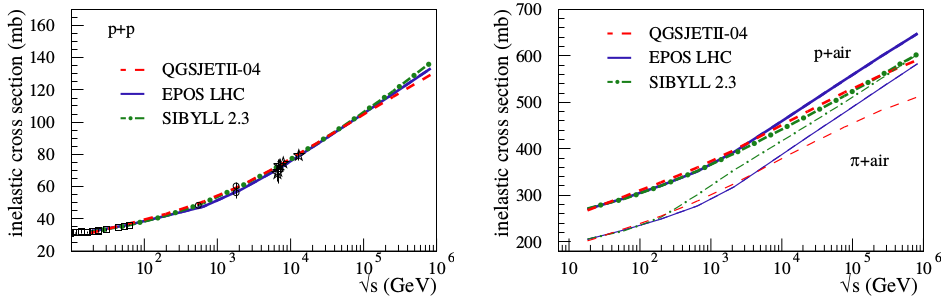
\includegraphics[width=0.95\textwidth]{Figuras/Pierog2018} 
\caption{Sección eficaz inelástica para interacciones p-p (izquierda) e interacciones p-aire y $\pi$-aire (derecha) calculadas con tres modelos hadrónicos \cite{Pierog2018}.}
\label{fig:cross_sections}
\end{figure}	

Por otro lado, otras observables que pueden ser fuente de información sobre la composición primaria de los rayos cósmicos son las distribuciones laterales de partículas (densidad de partículas a nivel de suelo en función de la distancia radial a partir del eje de la cascada) o la densidad de partículas a cierta distancia. Usualmente la distancia a la que se estudia la señal o la densidad de partículas es propia de cada observatorio y se denomina \textit{distancia óptima} ($r_{\text{opt}}$) \cite{Newton2007}, que se define como la distancia a la cual se minimizan las fluctuaciones estadísticas del ajuste de los datos a una función de distribución lateral. Estas mediciones se utilizan principalmente para determinar la energía inicial y la posición del eje del chubasco. \\

Distribuciones laterales de diversas partículas han sido medidas por varios experimentos; el experimento KASCADE (\textit{KArlsruhe Shower Core and Array DEtector}) ha realizado medidas de distribuciones laterales de electrones, muones y hadrones \cite{Antoni2001}, encontrando que los datos pueden describirse por funciones de tipo NKG. Asimismo, el PAO ha contemplado una función de distribución lateral de la señal en eventos detectados por su arreglo superficial \cite{Barnhill2005}, concluyendo -luego de ajustar los datos a diferentes funciones- que una función de tipo NKG (Nishimura-Kamata-Greisen) provee el mejor ajuste, y determinando $r_{\text{opt}} = 1000$ m para el observatorio. Más recientemente se han reportado resultados preliminares de AMIGA (\textit{Auger Muons and Infill for the Ground Array}), una extensión del PAO, donde se ha medido directamente la densidad de muones en cascadas \cite{Muller2019}, confirmando que los modelos de interacción hadrónica no reproducen correctamente los datos en el rango de las UHE. \\

Comparando datos experimentales con simulaciones se han interpretado datos de AGASA (\textit{Akeno Giant Air Shower Array}) de distribuciones laterales de electrones, fotones y muones; los resultados de simulaciones describen bien los datos, independientemente del modelo hadrónico y la composición primaria \cite{Nagano2000}. Tambi\'en se han comparado datos de KASCADE con simulaciones hechas con distintos modelos de interacción hadrónica y se mostró que las distribuciones de muones se reproducen bien, contrario a las de electrones que difieren de los datos experimentales \cite{Apel2005}, además se observó que ésta última sugiere un cambio a una composición pesada en el espectro de rayos cósmicos. \\

\begin{figure}[]
\centering
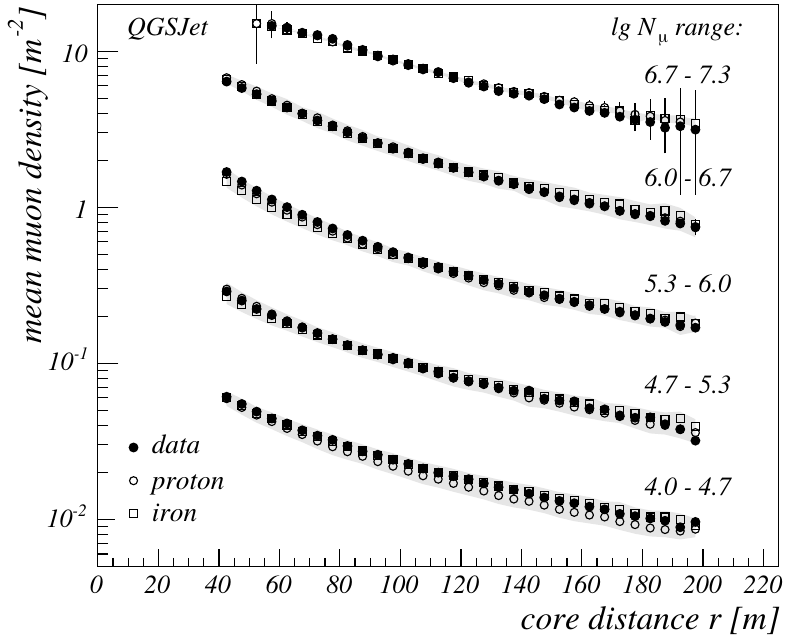
\includegraphics[width=0.6\textwidth]{Figuras/Apel2005} 
\caption{Comparación de distribuciones laterales de muones resultado de simulaciones con el programa CORSIKA y medidas del observatorio KASCADE \cite{Apel2005}.}
\label{fig:Apel}
\end{figure}


Igualmente se ha estudiado el impacto del modelo de interacciones hadrónicas en las funciones de distribución lateral a partir de datos experimentales. Por ejemplo, en \cite{Drescher2003} han comparado distintas combinaciones de modelos y concluyen que las funciones son dependientes de los modelos hadrónicos de bajas y altas energías. Asimismo, se ha explorado la relación entre la forma de las distribuciones laterales y la composición primaria de los UHECR; haciendo predicciones teóricas \cite{Raikin2001} y comparando con datos de AGASA se ha visto una alta dependencia de la función de distribución lateral con la energía y composición primarias, describiéndola con la variación del parámetro radio medio cuadrado $R_{m.s}$. \\

\begin{figure}[]
\centering
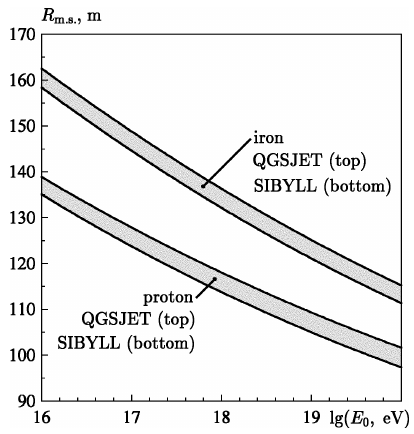
\includegraphics[width=0.5\textwidth]{Figuras/Raikin2001}
\caption{Radio medio cuadrado de electrones predicho teóricamente utilizando el formalismo de escala junto con modelos de interacción hadrónica utilizando el programa CORSIKA, mostrando su dependencia de la masa primaria \cite{Raikin2001}.}
\label{fig:Raikin}
\end{figure}

De manera que los modelos de interacci\'on hadr\'onica m\'as utilizados se han estudiado en t\'erminos de su impacto en ciertas caracter\'isticas de las cascadas atmosf\'ericas simuladas y su respectiva comparaci\'on con datos experimentales a energ\'ias $>10^{15}$ eV. No obstante a menores energ\'ias, en el rango de los TeV, tambi\'en se han reportado estudios de las diferencias entre modelos para algunas observables de las cascadas, donde se concluye que hay buena concordancia entre ellos para energ\'ias mayores que 10 TeV \cite{Parsons2019}. \\

El experimento HAWC es un ejemplo de observatorio a nivel de suelo que detecta part\'iculas producidas en cascadas atmosf\'ericas en el rango de los TeV utilizando sus 300 detectores de agua Cherenkov (WCDs por sus siglas en ingl\'es \textit{Water Cherenkov Detectors}) distribuidos en un \'area de $22000$ m$^2$ a una altura de 4100 m sobre el nivel del mar. Originalmente HAWC est\'a dise\~nado para estudiar rayos gamma, pero tambi\'en pueden estudiarse rayos c\'osmicos de hasta $10^{15}$ eV a trav\'es de las distribuciones laterales de las part\'iculas producidas en las cascadas.  Dichas distribuciones pueden contener informaci\'on sobre la part\'icula primaria como su energ\'ia y su masa. \\

Las observaciones de cascadas atmosf\'ericas en HAWC se han utilizado para medir diversas propiedades de los rayos c\'osmicos; se han confirmado y mejorado mediciones de la anisotrop\'ia en la direcci\'on incidente del flujo de los rayos c\'osmicos \cite{Abeysekara2018a}, el estudio de esta propiedad permite profundizar en la descripci\'on de la propagaci\'on de las part\'iculas a trav\'es de diferentes medios; tambi\'en se han extendido a mayores energ\'ias las mediciones del flujo de antiprotones \cite{Abeysekara2018} ayud\'andose del estudio del efecto lunar en el flujo de los rayos c\'osmico, imponiendo un l\'imite superior a la raz\'on $\bar{p}/p$ en el rango de 1-10 TeV; asimismo, se han observado potenciales fuentes de rayos c\'osmicos de origen gal\'actico además de remanentes de supernova \cite{Hooper2017, Malone2019, Abeysekara2021}.
%Un parrafo sobre el trabajo de HAWC sobre rayos cosmicos de TeV: mediciones de la anisotropia, medici[on del flujo de anti protones utilizando la sobra de la luna, Estudio de fuentes galacticas de rayos cosmicos.
\singlespace




\chapter{Metodología}
\spacing{1.25}
\section{Simulaciones de chubascos producidos por UHECR}
Se estudió el efecto de la composición primaria de los rayos cósmicos en la distribución lateral de electrones y muones y en la densidad de los mismos a una distancia de 1000 m del eje del chubasco. Para ello, con el programa AIRES se realizaron tres grupos de simulaciones por cada modelo de interacciones hadrónicas: el primer grupo de chubascos producidos por protones, el segundo chubascos producidos por hierro y el tercero chubascos producidos por una mezcla de protones, helio, nitrógeno y hierro. Cada grupo consistió en aproximadamente 2400 chubascos con ultraaltas energías, debido a que actualmente el problema de la composición se encuentra en esta región del espectro. 

	\subsection{Características de los chubascos}
	 Se simularon chubascos producidos por rayos cósmicos de energías entre $10^{17}$ y $10^{20}$ eV, en la ubicación de Malargue en Mendoza, Argentina -donde se encuentra una de las estaciones del PAO-. Se consideraron direcciones de incidencia con ángulo zenital entre 0$^{o}$ y 70$^{o}$ y ángulo azimutal distribuido isotrópicamente entre 0$^{o}$ y 360$^{o}$. Se utilizaron tres modelos de interacciones hadrónicas de altas energías; Sibyll 2.3c, EPOS-LHC y QGSJETII-04. Los tres se han destinado a este tipo de simulaciones anteriormente, y son precisamente dichos modelos los que muestran discrepancias en la composición de los UHECR basada en la profundidad $X_{\text{max}}$. \\
	 
	 En el rango de energías mencionado, se hicieron simulaciones de chubascos producidos únicamente por protones, producidos únicamente por núcleos de hierro y finalmente producidos por la composición primaria mixta, como propone la colaboración Pierre Auger \cite{PAOcomposition}, mostrada en la Fig. \ref{fig:composition}.
	 
\begin{center}
\begin{figure}[h]
\centering
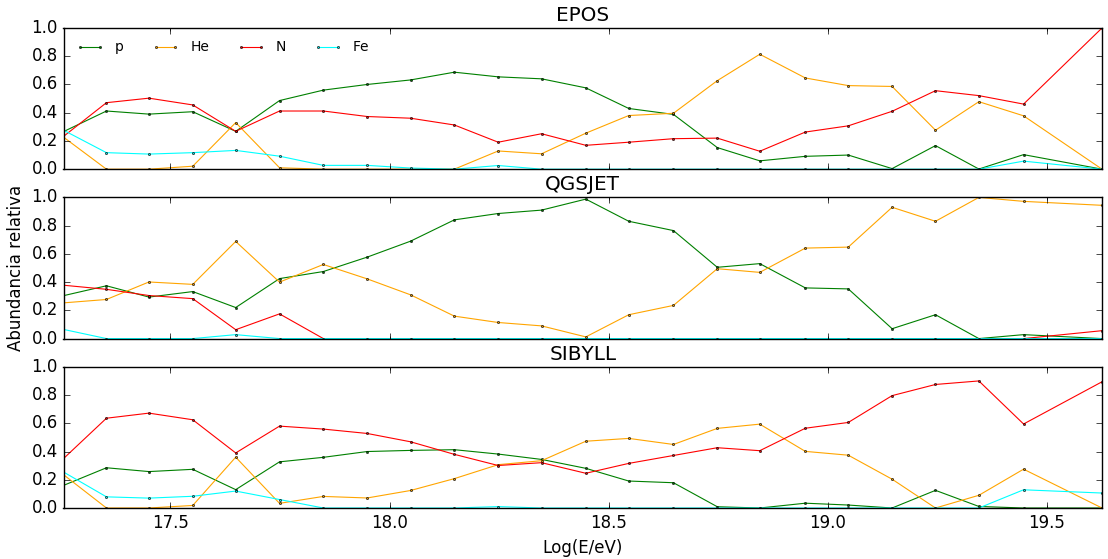
\includegraphics[height=0.3\textheight]{Figuras/composition.png} 
\caption{Composición en función de la energía, resultado de ajustes con los datos de $X_{\text{max}}$ del Observatorio Pierre Auger realizados con tres modelos de interacciones hadrónicas de altas energías.}
\label{fig:composition}
\end{figure}	
\end{center}

\section{Software para simulaciones de altas energías}
El sistema AIRES (AIR shower Extended Simulations) es un conjunto de programas para simular chubascos atmosféricos extendidos desarrollado por el Departamento de Física de la Universidad Nacional de La Plata y el Instituto de Física La Plata. AIRES está diseñado de manera modular para facilitar el intercambio entre los modelos de distintos aspectos de las simulaciones. El código completo de AIRES incluye los paquetes de interacciones hadrónicas EPOS 1.99, EPOS LHC, QGSJET-II-03, QGSJET-II-04, SIBYLL 2.1, SIBYLL 2.3, y SIBYLL 2.3c, así como las rutinas para evaluar el campo geomagnético. En síntesis, el sistema AIRES consiste en:
	\begin{itemize}
	\item Los programas de simulación principales (AiresEPLHC, AiresEP199, AiresQIIr03, AiresQIIr04, AiresS21, AiresS23, AiresS23c), cada uno conteniendo la interfaz para un paquete de interacciones hadrónicas.
	\item El programa resumen (AiresSry), diseñado para procesar parte de los datos generados por los programas de simulación.
	\item El programa de conversión de formato IDF (\textit{internal dump file}) a ADF (\textit{portable dump file}) (AiresIDF2ADF).
	\item Una librería de auxiliares para procesar los archivos de salida de los programas de simulación (libAires.a)
	\item El \textit{AIRES runner system}, para facilitar el trabajo con AIRES en ambientes UNIX. 
	\end{itemize}
	
	
	\subsection{Sistema de coordenadas}
	\begin{wrapfigure}{r}{0.3\textwidth}
	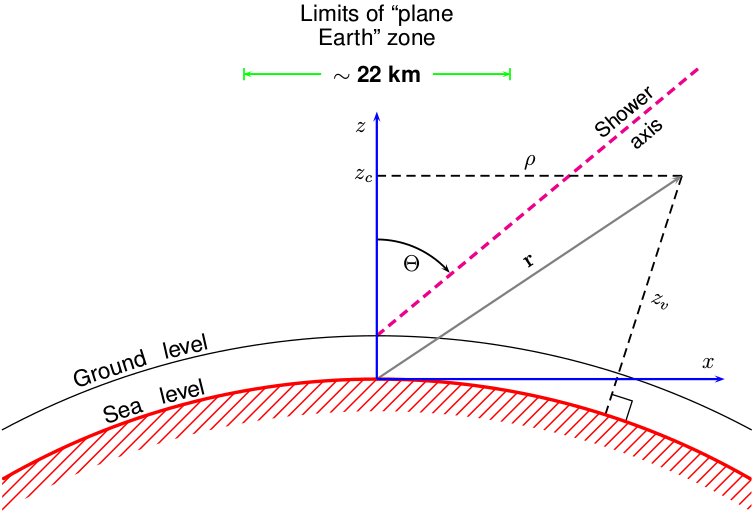
\includegraphics[width=0.3\textwidth]{Figuras/coordinates} 
	\caption{Esquema del sistema de coordenadas utilizado en AIRES.}
	\label{fig:coordinates}
	\end{wrapfigure}		
	El sistema de coordenadas de AIRES es un sistema cartesiano con el origen al nivel del mar en la ubicación proporcionada por el usuario, el plano $xy$ se posiciona horizontalmente; el eje $x$ apunta hacia el norte magnético, el eje $y$ hacia el Este y el eje $z$ hacia arriba. En la figura \ref{fig:coordinates} se muestra una representación esquemática del sistema coordenado, incluyendo el nivel del suelo y el nivel de inyección, éstos se refieren a superficies esféricas concéntricas con la superficie del nivel del mar. El eje del chubasco se define como una línea recta que pasa por la intersección del nivel del suelo con el eje $z$, con un ángulo cenital $\Theta$ y un ángulo azimutal $\Phi$.
	
	\subsection{Atmósfera}
	AIRES utiliza el modelo basado en datos experimentales \textit{US standard atmosphere} como modelo predeterminado. En este modelo, la composición de la atmosféra es $78.47\%$ N, $21.05\%$ O, $0.47\%$ Ar y $0.03\%$ otros elemento. El perfil de densidad isotérmico de la forma
	\begin{align*}
	\rho (h) = \rho_0 e^{-gMh/RT},
	\end{align*}
	
	se adapta a los valores de la \textit{US standard atmosphere}. En AIRES el modelo se extiende hasta una altura $h_{max} \sim 420$ km, después de la cual se considera que la densidad es cero. Se utiliza una parametrización de la profundidad atmosférica vertical $X_v$; dividiendo la atmósfera en $L$ capas, $X_v (h)$ se define por 
	\begin{align}
	X_v (h) = \begin{cases}
	a_l + b_l e^{-h/c_l} & h_l \leq h < h_{l+1} \\
	a_L - b_L (h/c_L) & h_L \leq h < h_{L+1} \\
	0 & h \geq h_{L+1}.
	\end{cases}
	\end{align}
	
	Los coeficientes usados en AIRES, que corresponden a un modelo con $L=5$, se muestran en la tabla. La profundidad atmosférica inclinada (\textit{slant}) $X_s$ depende del ángulo cenital y cuando no se toma en cuenta la curvatura de la Tierra, se relaciona con $X_v$ de la siguiente manera:
	\begin{align}
	X_s (h) = \frac{X_v (h)}{\cos(\Theta)}.
	\end{align}
	
	\subsection{Campo geomagnético}
	El campo magnético de la Tierra $\vb{B}$ se define por su intensidad $F$; su inclinación $I$, que se define como el ángulo entre el plano horizontal y el vector $\vb{B}$; y su declinación $D$, que se define como el ángulo entre la componente horizontal ($H$) de $\vb{B}$ y el norte geográfico. Las componentes cartesianas de $\vb{B}$ con respecto al sistema coordenado de AIRES son 
	\begin{align}
	B_x &= F \cos I, \\
	B_y &= 0, \\
	B_z &= -F \sin I.
	\end{align}	 
	
	Hay dos maneras de especificar el campo geomagnético en AIRES; la primera es ingresando manualmente los valores de $F$, $I$ y $D$, y la segunda es ingresando las coordenadas geográficas del lugar y la fecha para evaluar el campo magnético utilizando el modelo \textit{International Geomagnetic Reference Field} (IGRF).  	
	
	%\subsection{Modelos de interacción}
	%En AIRES se toman toman en cuenta los procesos más relevantes; procesos electrodinámicos como producción de pares (para $e^{\pm}$ y $\mu^{\pm}$), \textit{Bremsstrahlung}, efecto fotoeléctrico y efecto Compton; procesos hadrónicos como colisiones hadrón-núcleo, reacciones fotonucleares y fragmentación nuclear; procesos de decaimiento y procesos de propagación. \\
	
	%Cada interacción posible está caracterizada por su sección eficaz $\sigma_i$ o por su camino libre medio $\lambda_i$. Los caminos libres medios dependen del tipo de interacción y los parámetros instantáneos de la partícula. AIRES puede calcular $\lambda_i$ analíticamente para algunas interacciones , y en otros casos debe recurrir a modelos basados en datos experimentales. 
	
	\subsection{Estructura de los programas de simulación}
	Un chubasco se origina cuando un rayo cósmico interactúa con la atmósfera terrestre, donde se producen partículas secundarias que se propagan y pueden interactuar de manera similar produciendo más partículas. Eventualmente la multiplicidad de partículas llega a un máximo, después del cuál el chubasco empieza a atenuarse. En AIRES todo este proceso se simula de la siguiente manera \cite{Sciutto2002}:
	\begin{itemize}
	\item Se definen arreglos vacíos destinados a almacenar los datos de las características de las partículas.
	\item Las partículas pueden moverse por la atmósfera en un volumen delimitado por la superficie de inyección, el suelo y planos verticales que delimitan la región de interés.
	\item La primera acción es añadir a un arreglo la entrada correspondiente a la partícula inicial, ésta se localiza inicialmente en la superficie de inyección y su dirección de movimiento define el eje del chubasco.
	\item Las entradas respectivas a cada partícula se actualizan primero evaluando las probabilidades de todas las interacciones posibles.
	\item Se selecciona entre las posibles interacciones utilizando un método estocástico.
	\item Se procesa la interacción; la partícula se mueve una cierta distancia dependiente de la interacción seleccionada y luego se generan los productos de dicha interacción. Se agregan a los arreglos las entradas de las nuevas partículas creadas.
	\item En el caso de las partículas cargadas, se modifica la energía para tomar en cuenta pérdidas por ionización.
	\item Las entradas de partículas pueden removerse (1) si su energía es menor que cierto límite, (2) si alcanza el nivel del suelo, (3) si alcanza la superficie de inyección hacia arriba y (4) si horizontalmente sale de la región de interés.
	\item Se verifica que todas las entradas de partículas de los arreglos se hayan procesado; cuando se hayan procesado se completa la simulación del chubasco.
	\end{itemize}	
	
	\subsection{Muestreo de partículas}
	Para chubascos iniciados por partículas de ultraalta energía, el número de partículas secundarias producidas es tan grande que la tarea computacional de propagarlas todas es imposible; para poder realizar las simulaciones se emplea un mecanismo de muestreo que permite propagar únicamente un fracción representativa del total de partículas secundarias. AIRES utiliza una extensión del \textit{Hillas thinning algorithm} \cite{Kobal2001}. \\
	
	Considerando un proceso donde una partícula primaria $A$ genera un conjunto de $n$ secundarios, éstos son propagados con cierta probabilidad $P_i$. El algoritmo de Hillas consiste en establecer una constante $E_{th}$ llamada \textit{thinning energy}; para incorporar a los secundarios $B_i$ en la propagación se compara la energía de la partícula primaria $E_A$ con $E_{th}$: si $E_A \geq E_{th}$, entonces los secundarios de aceptan con una probabilidad
	\begin{align}
	P_i = \begin{cases}
	1 & \text{ si } E_{B_i} \geq E_{th} \\
	\frac{E_{B_i}}{E_{th}} & \text{ si } E_{B_i} < E_{th}.
	\end{cases}
	\end{align}
	Por el contrario, si $E_A < E_{th}$ sólo una partícula secundaria se conserva, lo que asegura que una vez se alcance $E_{th}$ el número de partículas no se incrementa. El algoritmo utilizado por AIRES es una extensión de lo descrito anteriormente, pero éste incluye características adicionales para disminuir las fluctuaciones estadísticas.

\singlespacing

\chapter{Resultados}
\spacing{1.25}
En este capítulo se presentan los resultados de las simulaciones de chubascos iniciados por rayos cósmicos de energías entre $10^{17.256}$ y $10^{19.626}$ eV, considerando la composición mixta de rayos cósmicos primarios basada en datos del Observatorio Pierre Auger. Se muestran los resultados de dos observables: la profundidad del máximo y su desviación estándar. Se comparan tres modelos de interacción hadrónica con los que se realizaron las simulaciones, además de comparar los resultados obtenidos con los respectivos datos observacionales. \\

Se simularon 2400 chubascos en el rango de energías mencionado, en la ubicación de Malargue -donde se encuentra una de las estaciones del Pierre Auger-, con ángulo zenital entre 0$^{o}$ y 70$^{o}$ y ángulo azimutal distribuido isotrópicamente entre 0$^{o}$ y 360$^{o}$. La simulaciones se realizaron con tres modelos de interacción hadrónica: Sibyll 2.3c, EPOS-LHC y QGSJETII-04, tomando en cuenta la composición primaria mixta (una combinación de protones, núcleos de helio, nitrógeno y hierro) propuesta por la colaboración Pierre Auger en \cite{PAOcomposition}, mostrada en la Fig. \ref{fig:composition}.

\begin{center}
\begin{figure}[h]
\centering
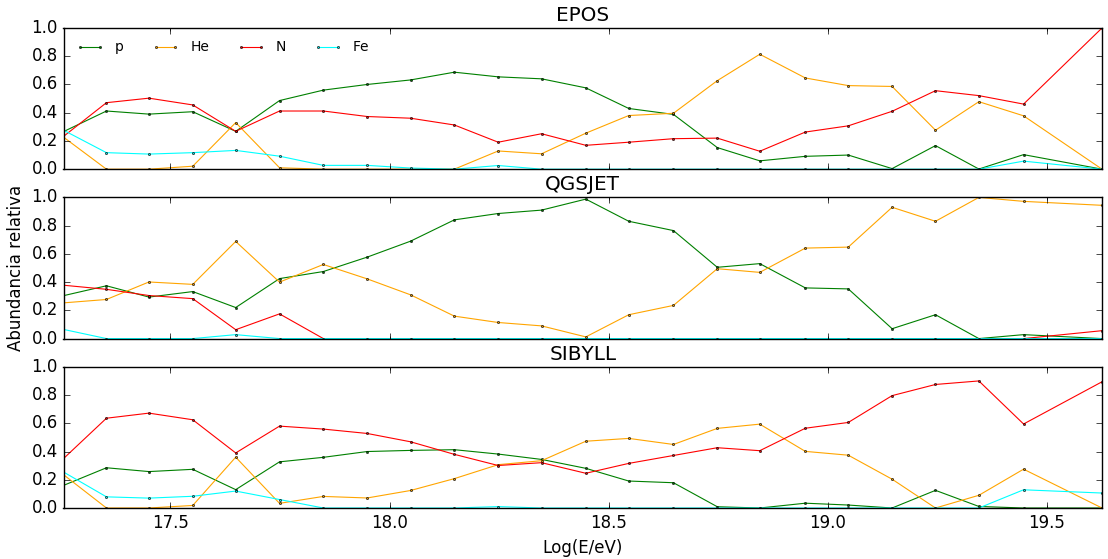
\includegraphics[height=0.3\textheight]{Figuras/composition} 
\caption{Composición en función de la energía, resultado de un ajuste con los datos del Observatorio Pierre Auger.}
\label{fig:composition}
\end{figure}	
\end{center}

\section{Profundidad del máximo $X_{max}$}
\subsection{Comparación de predicciones de los modelos hadrónicos}
Se calculó el promedio de la profundidad del máximo de 100 eventos para cada energía realizando el correspondiente ajuste mediante el algoritmo de mínimos cuadrados no lineal Levenberg-Marquardt. En la gráfica de la Fig. \ref{fig:Xmodelos} se muestran los resultados de $X_{max}$ para los tres modelos hadrónicos.\\

\begin{figure}[h]
\centering
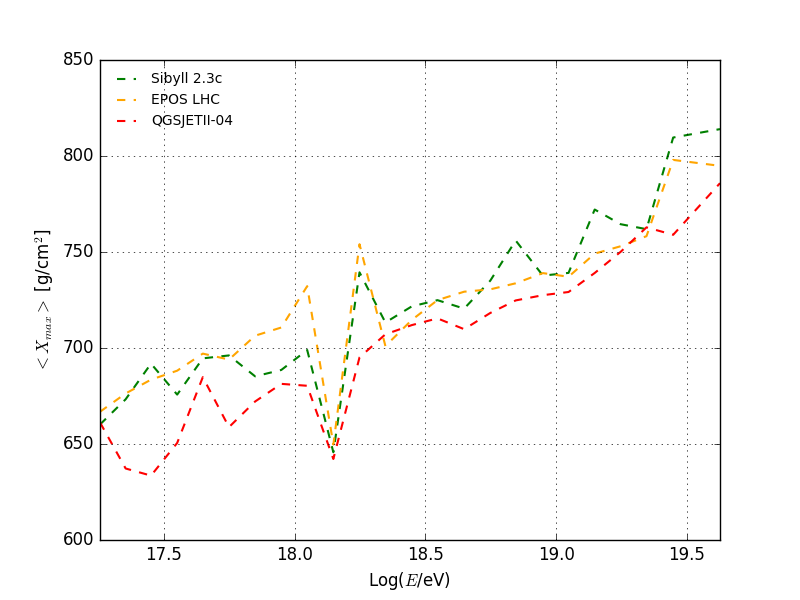
\includegraphics[width=0.7\textwidth]{Figuras/Xmax_modelos} 
\caption{$X_{max}$ promedio resultante de las simulaciones con los modelos hadrónicos Sibyll 2.3c, EPOS-LHC y QGSJETII-04}
\label{fig:Xmodelos}
\end{figure}	

Se observa que en general los tres modelos muestran la misma tendencia de crecimiento de $X_{max}$ con la energía, sin embargo el modelo QGSJET es el que más difiere de los otros dos modelos, prediciendo el máximo a una menor profundidad, con una diferencia promedio de aproximadamente 3\%, mientras que Sibyll y EPOS difieren entre ellos un 1.5\% en promedio.

\begin{table}[h]
\centering
\caption{Diferencias porcentuales entre los resultados de $X_{max}$ de los distintos modelos de interacción hadrónica.}
\begin{tabular}{l|ccc}
\hline
              & \multicolumn{1}{l}{Dif. media (\%)} & \multicolumn{1}{l}{Mín. (\%)} & \multicolumn{1}{l}{Máx. (\%)} \\ \hline
Sibyll/QGSJET & 2.914                               & 0.123                         & 9.207                         \\ \hline
EPOS/QGSJET   & 3.085                               & 0.379                         & 8.484                         \\ \hline
Sibyll/EPOS   & 1.473                               & 0.003                         & 4.544  						  \\ \hline 
\end{tabular}
\label{modeldif} 
\end{table}

\subsection{Comparación con datos observacionales}
En la figura Fig. \ref{fig:Xobs} se muestran tanto los resultados de las simulaciones como los datos obtenidos por el Observatorio Pierre Auger. Los modelos Sibyll y EPOS muestran excelente concordancia con las observaciones en las energías más bajas del rango considerado, luego de $E\approx 10^{18.248}$ eV los datos simulados son en general menores que los experimentales. Por otro lado, QGSJET tiende a subestimar la profundidad del máximo de los chubascos en todo el rango de energías.\\

\begin{figure}[h]
\centering
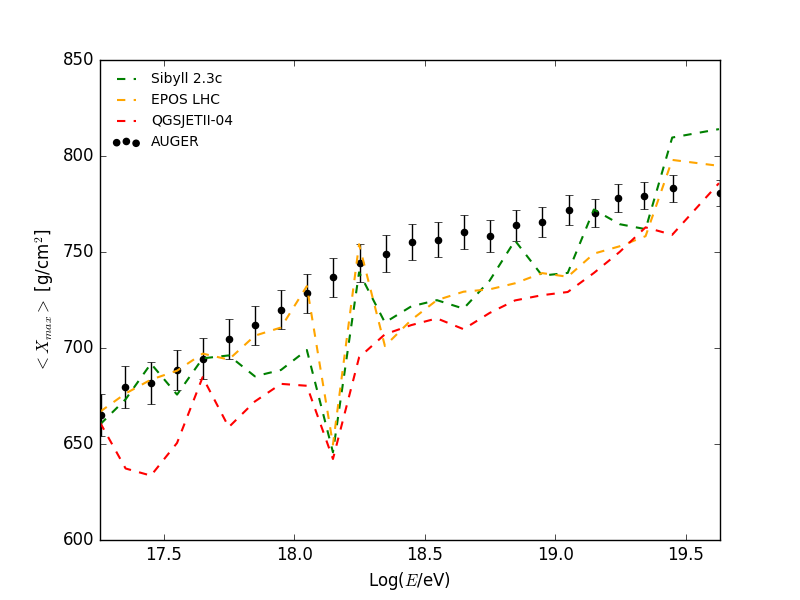
\includegraphics[width=0.7\textwidth]{Figuras/Xmax_modelos_obs} 
\caption{$X_{max}$ promedio resultante de las simulaciones con los modelos hadrónicos Sibyll 2.3c, EPOS-LHC y QGSJETII-04 junto con los datos tomados por el Observatorio Pierre Auger. Las barras representan el error sisteático de las medidas.}
\label{fig:Xobs}
\end{figure}	

Para toda la ventana de energías, el modelo EPOS es el que mejor reproduce los datos del Pierre Auger, con un error relativo de 2.8\% en promedio, le sigue Sibyll con 3.1\% y por último está QGSJET con 5.1\% de error relativo.\\

\begin{table}[h]
\centering
\caption{Error porcentual de los resultados de $X_{max}$ de las simulaciones relativo a los datos observacionales.}
\begin{tabular}{l|ccc}
\hline
Modelo & Err. relativo (\%) & Mín. (\%) & Máx. (\%) \\ \hline
Sibyll & 3.080              & 0.023     & 12.364    \\ \hline
EPOS   & 2.778              & 0.050     & 11.820    \\ \hline
QGSJET & 5.092              & 0.589     & 12.840    \\ \hline
\end{tabular}
\end{table}

La subestimación de $X_{max}$ en las simulaciones puede sugerir que en las mayores energías, los chubascos se producen por rayos cósmicos de composición más ligera que la que se ha considerado. Sin embargo, como evidencian las discrepancias entre los modelos, la reproducción de los datos observacionales es altamente dependiente del modelo hadrónico utilizado y de sus características particulares.


\section{Desviación estándar del máximo $\sigma X_{max}$}
\subsection{Comparación de predicciones de los modelos hadrónicos}
Las fluctuaciones de la profundidad del máximo de un chubasco a otro con la misma energía es una magnitud que también es sensible a la composición primaria. En la Fig. \ref{fig:Smodelos} se muestran los resultados de las simulaciones para esta observable. \\

\begin{figure}[h]
\centering
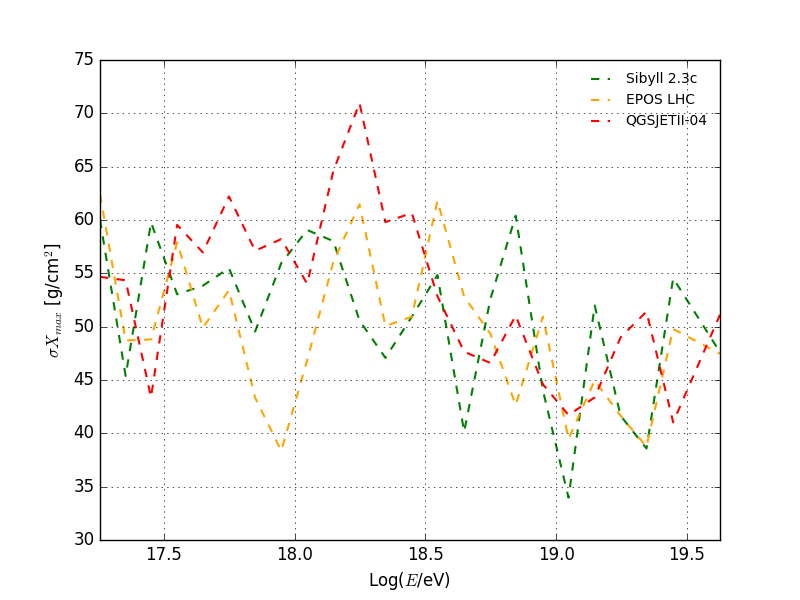
\includegraphics[width=0.7\textwidth]{Figuras/StddvXmax_modelos} 
\caption{Fluctuaciones en el valor de profundidad del máximo $\sigma X_{max}$ resultante de las simulaciones con los modelos hadrónicos Sibyll 2.3c, EPOS-LHC y QGSJETII-04.}
\label{fig:Smodelos}
\end{figure}	

En el caso de $\sigma X_{max}$ se observa que los tres modelos hadrónicos difieren de manera notable entre sí. Las diferencias se encuentran alrededor de 15\% en casi todo el rango de interés, a pesar de coincidir en puntos aislados. No se observa una tendencia clara de los datos simulados.

\begin{table}[h]
\centering
\caption{Diferencias porcentuales entre los resultados de $\sigma X_{max}$ de los distintos modelos de interacción hadrónica.}
\begin{tabular}{l|ccc}
\hline
              & Dif. media (\%) & Mín. (\%) & Máx. (\%) \\ \hline
Sibyll/QGSJET & 15.168          & 1.256     & 37.782    \\ \hline
EPOS/QGSJET   & 14.089          & 2.721     & 34.101    \\ \hline
Sibyll/EPOS   & 12.651          & 0.000     & 45.881    \\ \hline
\end{tabular}
\end{table}

\subsection{Comparación con datos observacionales}
En la Fig. \ref{fig:Sobs} se muestran los datos experimentales $\sigma X_{max}$ junto con los resultados de las simulaciones. Es evidente que el modelo que mejor reproduce la tendencia de los datos es QGSJET, principalmente en la parte central del rango desde $\sim 10^{17.551}$ hasta $\sim 10^{18.845}$. En las menores energías QGSJET subestima las fluctuaciones, mientras que en las mayores las sobreestima. Las predicciones de EPOS y Sibyll están en general más bajas que los datos, con excepción de las mayores energías donde los tres modelos están por encima de los datos de l Pierre Auger.\\

\begin{figure}[h]
\centering
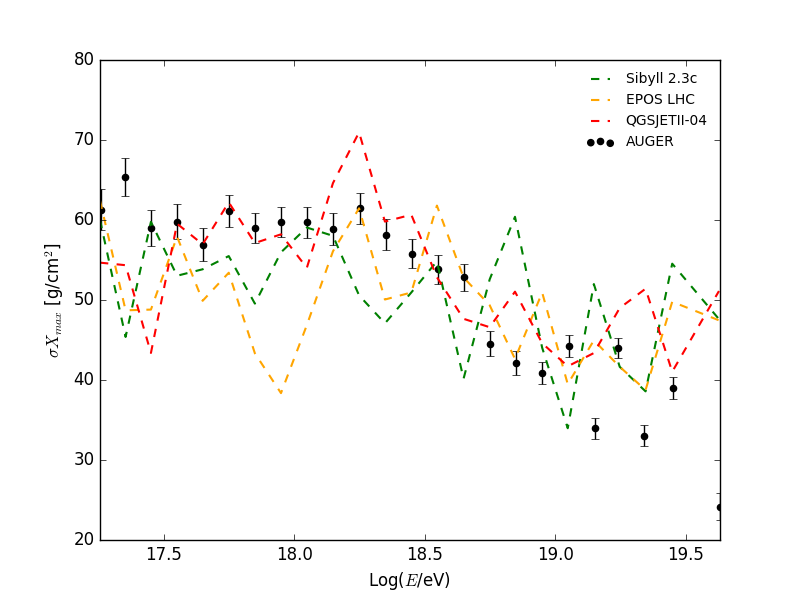
\includegraphics[width=0.7\textwidth]{Figuras/StddvXmax_modelos_obs} 
\caption{Fluctuaciones en el valor de profundidad del máximo $\sigma X_{max}$ resultantes de las simulaciones con los modelos hadrónicos Sibyll 2.3c, EPOS-LHC y QGSJETII-04 junto con los datos tomados por el Observatorio Pierre Auger. Las barras representan el error sisteático de las medidas.}
\label{fig:Sobs}
\end{figure}	

Ninguno de los tres modelos hadrónicos utilizados reproduce fielmente la desviación estándar de la profundidad del máximo, con errores del 18\% en promedio pero que llegan a ser de más del 30\% en varios puntos. Esto puede deberse principalmente a la cantidad de chubascos simulados con una misma energía, que está bastante por debajo de la cantidad de eventos observados a bajas energías, y por el contrario está por encima de los eventos observados a más altas energías. De manera que la cantidad de simulaciones realizadas puede estar afectando las fluctuaciones de chubasco a chubasco, no obstante estas diferencias con los datos observacionales no parecen indicar un cambio claro en la composición primaria.

\begin{table}[h]
\centering
\caption{Error porcentual de los resultados de $\sigma X_{max}$ de las simulaciones relativo a los datos observacionales.}
\begin{tabular}{l|ccc}
\hline
Modelo & Err. relativo (\%) & Mín. (\%) & Máx. (\%) \\ \hline
Sibyll & 19.192             & 1.072     & 97.143    \\ \hline
EPOS   & 17.722             & 0.016     & 96.522    \\ \hline
QGSJET & 15.509             & 0.053     & 111.677   \\ \hline
\end{tabular}
\end{table}

\singlespacing

\chapter{Conclusiones y recomendaciones}
\spacing{1.25}

A partir de la hipótesis de la colaboración Pierre Auger, que sugiere que los rayos cósmicos primarios que entran a la atmósfera terrestre con ultraaltas energías tienen una composición mixta conformada por núcleos de hidrógeno, helio, nitrógeno y hierro, se han realizado simulaciones de chubascos iniciados por rayos cósmicos de dicha naturaleza, calculando magnitudes de los mismos que son sensibles a la masa de la partícula inicial: $X_{\text{max}}$, distribuciones laterales de electrones y muones, y sus densidades a una distancia de 1000 m del eje del chubasco. Reproduciendo resultados ya bien conocidos, la hipótesis de la composición mixta es apoyada por los resultados de $X_{\text{max}}$. \\

El modelo EPOS-LHC el que más acertadamente reproduce los datos observacionales de $X_{max}$ para todo el rango de las ultraaltas energías, no obstante incluso este modelo tiende a subestimar la profundidad de máximo para las energías más altas. Los otros dos modelos subestiman esta cantidad en un intervalo aun más amplio, siendo el modelo QGSJETII-04 el que predice menores profundidades debido a su baja multiplicidad en las interacciones hadrónicas con respecto a los otros dos modelos. \\

En el caso de las distribuciones laterales resultantes de chubascos de todo el intervalo de energías, los tres modelos producen formas similares pero QGSJETII-04 muestra menor densidad de partículas a nivel de suelo, sin embargo este efecto no es tan drástico cuando se consideran las distribuciones laterales de chubascos en un pequeño subintervalo de energía primaria. También se observa que al aumentar la energía la forma de las distribuciones se mantiene similar, aumentando en general el número de partículas. \\

El efecto de la composición primaria es contrario para electrones y muones, encontrando que los chubascos producidos por protones muestran más electrones, mientras los producidos por hierro muestran mayor cantidad de muones a nivel de suelo; no obstante, a energías primarias mayores las distribuciones de distintas composiciones casi se sobrelapan, por lo que se concluye que a las más altas energías del rango considerado, las distribuciones laterales de electrones y muones no son sensibles a la masa  de la partícula que inició el chubasco. \\

Por último, las densidades de partículas a la distancia óptima del PAO en función de la energía inicial no muestran una clara dependencia del modelo de interacciones hadrónicas, a pesar de que las razones entre modelos son más fluctuantes. La densidad de electrones no presenta dependencia tampoco de la composición primaria, mientras que la densidad de muones aumenta sus diferencias entre composiciones al aumentar la energía; las diferencias causadas por la composición se ilustran con los valores obtenidos del ajuste de los datos a una ley de potencias. \\

Cabe resaltar, finalmente, que la reproducción de datos experimentales de profundidad del máximo por medio de simulaciones computacionales en función de una única composición primaria mixta es altamente dependiente del modelo de interacción hadrónica utilizado. Lo anterior se evidencia en las diferentes proporciones de partículas en la composición propuestas para cada uno de los modelos, así como en las claras discrepancias entre los resultados de las simulaciones. Caso contrario, las distribuciones laterales y densidad de partículas a energías iniciales determinadas no tienen una dependencia significativa con los modelos, obteniendo resultados similares con los tres. Por lo que, a pesar de que el efecto de la composición primaria es menos notorio, estas magnitudes parecen prometedoras para investigar la composición primaria de los rayos cósmicos de ultraaltas energías mediante comparaciones entre simulaciones y observaciones. \\

Se propone como trabajo a futuro verificar el efecto de la composición primaria mixta en otras propiedades de los chubascos, como la producción de partículas secundarias (fotones, electrones o muones) y su distribución lateral e igualmente su desarrollo longitudinal, particularmente su profundidad de máxima producción, así como realizar comparaciones detalladas entre datos de detección de partículas producidas en chubascos y simulaciones. Se recomienda que se simule un mayor número de eventos que sea proporcional al espectro de UHECR medido, invirtiendo más recursos computacionales de los que se disponen actualmente.

\singlespacing

\printbibliography[title=Referencias]

\end{document}